\documentclass{article}
%% GRAPH OF TRAFFIC CIRCLE
\usepackage{tikz}
\usetikzlibrary{arrows}
\begin{document}
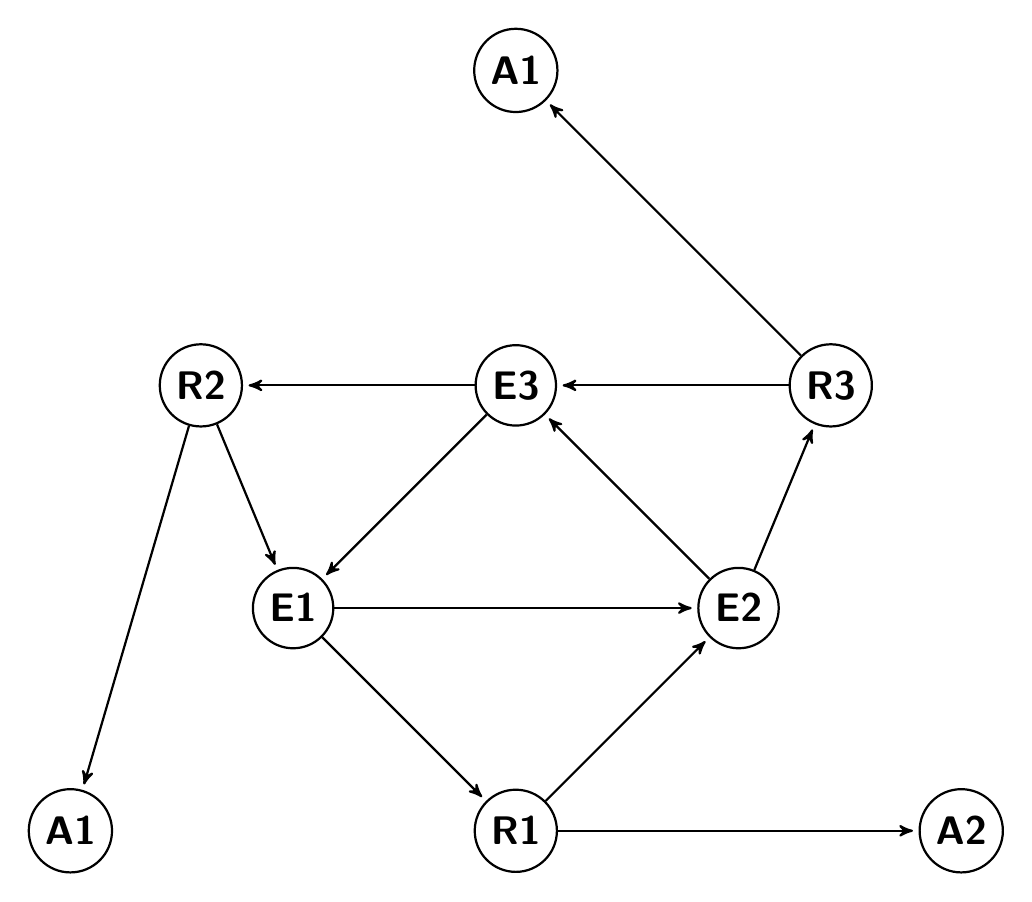
\begin{tikzpicture}[->, >=stealth', shorten >=2pt,auto,node distance=4cm, thick, main node/.style={circle, draw, font = \sffamily\Large\bfseries}]
\node[main node] (1){A1};
\node[main node](3)[below of=1]{E3};
\node[main node](2)[right of=3]{R3};
\node[main node](4)[left of=3]{R2};
\node[main node](5)[below left of=3]{E1};
\node[main node](6)[below right of=3]{E2};
\node[main node](7)[below left of=5]{A1};
\node[main node](8)[below right of= 5]{R1};
\node[main node](9)[below right of=6]{A2};


\path[every node/.style={font=\sffamily\small}]
(2) edge node {}(1)
     edge node {}(3)
(3) edge node{}(4)
     edge node{}(5)
(4) edge node{}(7)
     edge node{} (5)
(5) edge node{} (8)
     edge node{} (6)
(8) edge node{} (6)
     edge node{} (9)
(6) edge node{} (3)
     edge node{} (2);

\end{tikzpicture}
\end{document} 